\documentclass[a4paper,12pt]{article}
\usepackage[czech]{babel}
\usepackage[utf8]{inputenc}
\usepackage[T1]{fontenc}
\usepackage{graphicx}
\usepackage{hyperref}
\usepackage{geometry}
\geometry{margin=2.5cm}
\usepackage{setspace}
\usepackage{titlesec}
\usepackage{listings}
\usepackage{xcolor}
\usepackage{placeins}

% Nastavení pro zobrazování kódu
\definecolor{codegreen}{rgb}{0,0.6,0}
\definecolor{codegray}{rgb}{0.5,0.5,0.5}
\definecolor{codepurple}{rgb}{0.58,0,0.82}
\definecolor{backcolour}{rgb}{0.95,0.95,0.92}

\lstdefinestyle{mystyle}{
    backgroundcolor=\color{backcolour},   
    commentstyle=\color{codegreen},
    keywordstyle=\color{blue},
    numberstyle=\tiny\color{codegray},
    stringstyle=\color{codepurple},
    basicstyle=\ttfamily\footnotesize,
    breakatwhitespace=false,         
    breaklines=true,                 
    captionpos=b,                    
    keepspaces=true,                 
    numbers=left,                    
    numbersep=5pt,                  
    showspaces=false,                
    showstringspaces=false,
    showtabs=false,                  
    tabsize=2
}

\lstset{style=mystyle}

\titleformat{\section}{\large\bfseries}{\thesection}{1em}{}

\begin{document}

% --- Úvodní stránka ---
\begin{titlepage}
    \centering
    \vspace*{2cm}
    
    {\LARGE \textbf{Univerzita Jana Evangelisty Purkyně v Ústí nad Labem}}\\[0.5cm]
    {\Large \textbf{Přírodovědecká fakulta}}\\[0.5cm]
    {\Large \textbf{Katedra informatiky}}\\[3cm]

    {\Huge \textbf{OLAP a DuckDB}}\\[2cm]

    {\Large Seminární práce}\\[0.5cm]
    {\Large Rok: 2025}\\[3cm]

    \begin{flushright}
        {\Large Vypracoval: Valdemar Pospíšil}\\
    \end{flushright}
\end{titlepage}
\newpage

\tableofcontents
\newpage

% --- Hlavní část dokumentu ---
\section{Úvod do DuckDB}
DuckDB je moderní analytický databázový systém typu OLAP (Online Analytical Processing), který je navržen pro rychlé dotazování a analýzu velkých objemů dat. Na rozdíl od tradičních databázových systémů jako PostgreSQL nebo MySQL, které jsou primárně zaměřeny na OLTP (Online Transaction Processing), je DuckDB optimalizován pro analytické dotazy, které zpracovávají velké množství dat a provádějí agregace.

Mezi hlavní výhody DuckDB patří:
\begin{itemize}
    \item \textbf{Jednoduchost} - lze používat jako vestavěnou databázi bez nutnosti spouštění samostatného serveru
    \item \textbf{Rychlost} - optimalizovaný pro analytické dotazy a operace OLAP
    \item \textbf{Sloupcově orientované úložiště} - efektivní pro analytické dotazy, které často pracují s omezeným počtem sloupců
    \item \textbf{Integrace s Pythonem} - snadné použití v datových analýzách a vědeckých výpočtech
    \item \textbf{SQL kompatibilita} - plná podpora standardních SQL příkazů
\end{itemize}

\subsection{Instalace DuckDB na Linux}
Pro instalaci DuckDB na operačním systému Void Linux jsem použil správce balíčků pip pro Python. Instalace je jednoduchá a přímočará:

\begin{lstlisting}[language=bash, caption=Instalace DuckDB pomocí pip]
# Aktualizace pip
pip install --upgrade pip

# Instalace DuckDB
pip install duckdb
\end{lstlisting}

Na Linux možné si nainstalovat duckdb jakožto samostatný databázový server pomocí jednoduchého příkazu:

\begin{lstlisting}[language=bash, caption=Instalace duckdb na linux zařizeních pomocí příkazu]
# Instalace duckdb
curl https://install.duckdb.org | sh
\end{lstlisting}

\subsection{Vytvoření a použití databáze v DuckDB}

Vytvoření databáze v DuckDB je velmi jednoduché. Databázi lze vytvořit a používat přímo z Pythonu bez nutnosti spouštět samostatný databázový server:

\begin{lstlisting}[language=python, caption=Vytvoření a připojení k databázi v DuckDB]
import duckdb

# Vytvoreni pripojeni k databazi (pokud soubor neexistuje, bude vytvoren)
con = duckdb.connect("ufo.db")

# Vytvoření tabulky
con.execute("""
    CREATE TABLE example_table (
        id INTEGER PRIMARY KEY,
        name VARCHAR(100),
        value DOUBLE
    )
""")

# Vlozeni dat
con.execute("INSERT INTO example_table VALUES (1, 'Test', 10.5)")

# Dotaz
result = con.execute("SELECT * FROM example_table").fetchall()
print(result)

# Uzavreni pripojeni
con.close()
\end{lstlisting}

Databáze je uložena v souboru, který je specifikován při vytváření připojení. Pokud soubor neexistuje, DuckDB ho automaticky vytvoří. Tím se DuckDB liší od většiny databázových systémů, které vyžadují spuštění serveru.

\section{Dataset}
Pro projekt jsem si stáhl dataset \textbf{UFO Sightings} z Kaggle (\url{https://www.kaggle.com/datasets/sahityasetu/ufo-sightings}). Dataset obsahuje informace o pozorování UFO včetně času, místa, popisu a tvaru objektu.

Dataset obsahuje následující hlavní sloupce:
\begin{itemize}
    \item \textbf{Date\_time} - datum a čas pozorování
    \item \textbf{Date\_documented} - datum, kdy bylo pozorování zaznamenáno
    \item \textbf{Year}, \textbf{Month}, \textbf{Hour} - extrahované časové údaje
    \item \textbf{Season} - roční období
    \item \textbf{Country\_Code}, \textbf{Country}, \textbf{Region}, \textbf{Locale} - údaje o lokalitě
    \item \textbf{Latitude}, \textbf{Longitude} - geografické souřadnice
    \item \textbf{UFO\_shape} - tvar pozorovaného objektu
    \item \textbf{Length\_of\_encounter\_seconds} - doba trvání pozorování v sekundách 
    \item \textbf{Encounter\_Duration} - textový popis délky pozorování
    \item \textbf{Description} - podrobný popis pozorování
\end{itemize}

Pro načtení dat z CSV souboru do databáze jsem použil příkaz COPY:

\begin{lstlisting}[language=sql, caption=Načtení dat z CSV souboru]
-- Vytvoreni zakladni tabulky z CSV
CREATE TABLE sightings (
    Date_time TIMESTAMP,
    Date_documented DATE,
    Year INT,
    Month INT,
    Hour INT,
    Season VARCHAR(20),
    Country_Code VARCHAR(10),
    Country VARCHAR(100),
    Region VARCHAR(100),
    Locale VARCHAR(100),
    Latitude DOUBLE,
    Longitude DOUBLE,
    UFO_shape VARCHAR(50),
    Length_of_encounter_seconds BIGINT,
    Encounter_Duration VARCHAR(50),
    Description TEXT
);

-- Nacteni dat z CSV souboru s oddelovacem carkou
COPY sightings FROM 'ufo_sightings.csv' (DELIMITER ',', HEADER);
\end{lstlisting}

\section{Vytvoření datového skladu}
Vytvořil jsem datovou strukturu ve tvaru \textbf{hvězdy (star schema)} s jednou faktovou tabulkou a třemi dimenzními tabulkami. Tato struktura je typická pro OLAP analýzy a umožňuje efektivní dotazování na různých úrovních granularity.

\subsection{Dimenzní tabulky}
Dimenzní tabulky obsahují popisné atributy, které jsou využívány pro filtrování a seskupování dat:

\begin{itemize}
    \item \textbf{dim\_ufo}: obsahuje různé tvary UFO.
    \item \textbf{dim\_time}: obsahuje časové údaje (rok, měsíc, den, hodina).
    \item \textbf{dim\_location}: obsahuje údaje o zemi, regionu a lokalitě.
\end{itemize}

\subsection{Faktová tabulka}
Faktová tabulka obsahuje měřené hodnoty (fakta) a cizí klíče, které odkazují na dimenzní tabulky:

\begin{itemize}
    \item \textbf{fact\_sightings}: obsahuje jednotlivá pozorování, která jsou propojena na dimenze přes cizí klíče.
\end{itemize}

\subsection{SQL kód pro vytvoření struktury datového skladu}
Nejprve jsem musel vytvořit sekvence pro generování primárních klíčů:

\begin{lstlisting}[language=sql, caption=Vytvoření sekvencí]
-- Vytvoreni sekvenci pro primarni klice
CREATE SEQUENCE time_id_seq START 1;
CREATE SEQUENCE location_id_seq START 1;
CREATE SEQUENCE ufo_id_seq START 1;
CREATE SEQUENCE sighting_id_seq START 1;
\end{lstlisting}

Poté jsem vytvořil dimenzní tabulky:

\begin{lstlisting}[language=sql, caption=Vytvoření dimenzních tabulek]
-- Dimenzni tabulka pro cas
CREATE TABLE dim_time (
    time_id INTEGER DEFAULT nextval('time_id_seq') PRIMARY KEY,
    date_time TIMESTAMP,
    date_documented DATE,
    year INT,
    month INT,
    hour INT,
    season VARCHAR(20)
);

-- Dimenzni tabulka pro lokality
CREATE TABLE dim_location (
    location_id INTEGER DEFAULT nextval('location_id_seq') PRIMARY KEY,
    country_code VARCHAR(10),
    country VARCHAR(100),
    region VARCHAR(100),
    locale VARCHAR(100),
    latitude DOUBLE,
    longitude DOUBLE
);

-- Dimenzni tabulka pro tvary UFO
CREATE TABLE dim_ufo (
    ufo_id INTEGER DEFAULT nextval('ufo_id_seq') PRIMARY KEY,
    ufo_shape VARCHAR(50)
);
\end{lstlisting}

Následně jsem vytvořil faktovou tabulku, která obsahuje cizí klíče odkazující na dimenzní tabulky:

\begin{lstlisting}[language=sql, caption=Vytvoření faktové tabulky]
-- Faktova tabulka
CREATE TABLE fact_sightings (
    sighting_id INTEGER DEFAULT nextval('sighting_id_seq') PRIMARY KEY,
    time_id INT REFERENCES dim_time(time_id),
    location_id INT REFERENCES dim_location(location_id),
    ufo_id INT REFERENCES dim_ufo(ufo_id),
    length_of_encounter_seconds BIGINT,
    encounter_duration VARCHAR(50),
    description TEXT
);
\end{lstlisting}

\subsection{Naplnění dimenzních a faktové tabulky}
Po vytvoření tabulek jsem do nich naplnil data z původní tabulky \texttt{sightings}:

\begin{lstlisting}[language=sql, caption=Naplnění dimenzních tabulek]
-- Naplneni dimenzni tabulky casu
INSERT INTO dim_time (date_time, date_documented, year, month, hour, season)
SELECT DISTINCT Date_time, date_documented, Year, Month, Hour, Season
FROM sightings;

-- Naplneni dimenzni tabulky lokality
INSERT INTO dim_location (country_code, country, region, locale, latitude, longitude)
SELECT DISTINCT Country_Code, Country, Region, Locale, latitude, longitude
FROM sightings;

-- Naplneni dimenzni tabulky UFO
INSERT INTO dim_ufo (ufo_shape)
SELECT DISTINCT UFO_shape
FROM sightings;
\end{lstlisting}

Nakonec jsem naplnil faktovou tabulku, přičemž jsem vytvořil spojení s dimenzními tabulkami:

\begin{lstlisting}[language=sql, caption=Naplnění faktové tabulky]
-- Naplneni faktove tabulky
INSERT INTO fact_sightings (time_id, location_id, ufo_id, length_of_encounter_seconds, encounter_duration, description)
SELECT 
    t.time_id,
    l.location_id,
    u.ufo_id,
    s.length_of_encounter_seconds,
    s.Encounter_Duration,
    s.Description
FROM sightings s
JOIN dim_time t ON s.Date_time = t.date_time 
                AND s.date_documented = t.date_documented 
                AND s.Year = t.year 
                AND s.Month = t.month 
                AND s.Hour = t.hour 
                AND s.Season = t.season
JOIN dim_location l ON s.Country_Code = l.country_code 
                     AND s.Country = l.country 
                     AND s.Region = l.region 
                     AND s.Locale = l.locale 
                     AND s.latitude = l.latitude 
                     AND s.longitude = l.longitude
JOIN dim_ufo u ON s.UFO_shape = u.ufo_shape;
\end{lstlisting}

\section{Analytické dotazy}
Po vytvoření datového skladu jsem provedl několik analytických dotazů k získání zajímavých informací o pozorováních UFO. Dotazy byly implementovány v Pythonu s využitím knihovny DuckDB a výsledky byly vizualizovány pomocí knihoven jako \textbf{Matplotlib}, \textbf{Seaborn}, \textbf{Tabulate}, \textbf{Plotly} a \textbf{Folium}.

\subsection{Rozložení pozorování UFO podle států}
První analýza se zaměřila na počet pozorování UFO v jednotlivých státech USA. Implementoval jsem ji pomocí následujícího SQL dotazu:

\begin{lstlisting}[language=sql, caption=SQL dotaz pro počet pozorování podle států]
WITH state_sightings AS (
    SELECT
        l.region,
        f.length_of_encounter_seconds
    FROM fact_sightings f
    JOIN dim_location l ON f.location_id = l.location_id
    WHERE l.country_code = 'USA' AND l.region IS NOT NULL
)
SELECT
    region AS state,
    COUNT(*) AS sightings_count,
    AVG(length_of_encounter_seconds) AS avg_encounter_seconds,
    MEDIAN(length_of_encounter_seconds) AS median_encounter_seconds
FROM state_sightings
GROUP BY region
ORDER BY sightings_count DESC
\end{lstlisting}

Výsledky byly vizualizovány pomocí horizontálního sloupcového grafu a interaktivní choroplethové mapy pomocí knihovny Plotly.

\begin{figure}[h]
\centering
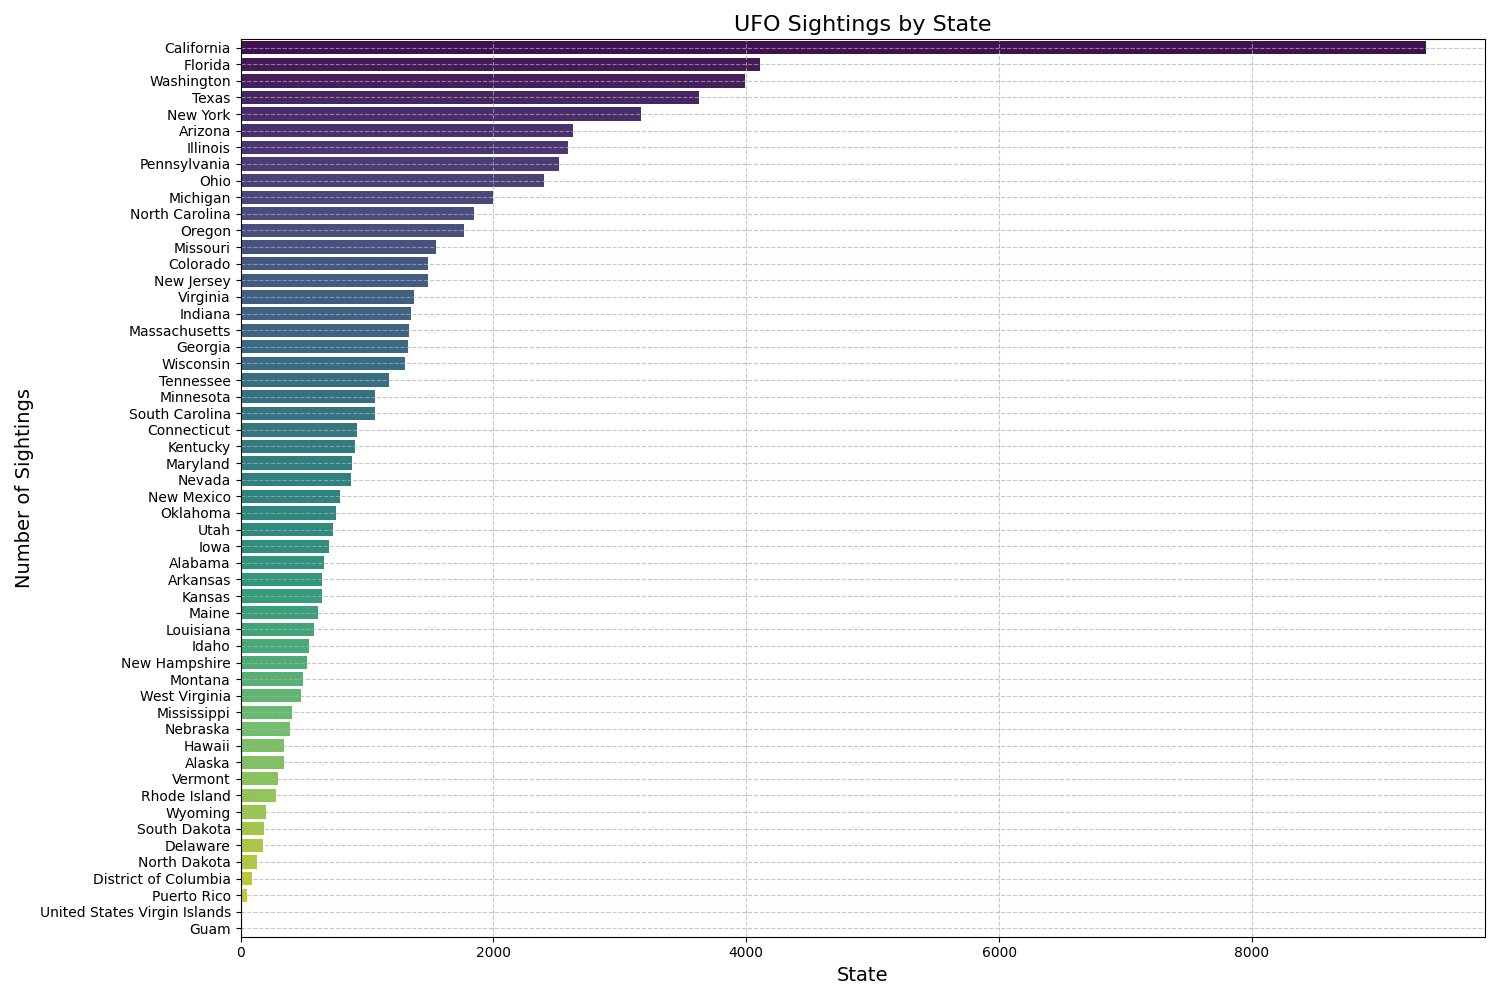
\includegraphics[width=0.8\textwidth]{../images/ufo_sightings_by_state.png}
\caption{Počet pozorování UFO podle států}
\end{figure}

\subsection{Distribuce délky pozorování}
Další analýza se zaměřila na délku pozorování UFO podle tvaru objektu. Implementoval jsem ji pomocí následujícího SQL dotazu:

\begin{lstlisting}[language=sql, caption=SQL dotaz pro délku pozorování podle tvaru UFO]
SELECT 
    d.ufo_shape,
    MEDIAN(f.length_of_encounter_seconds)::INTEGER AS median_seconds,
    COUNT(*) AS sightings_count,
    AVG(f.length_of_encounter_seconds)::INTEGER AS avg_seconds
FROM fact_sightings f
JOIN dim_ufo d ON f.ufo_id = d.ufo_id
WHERE f.length_of_encounter_seconds IS NOT NULL AND f.length_of_encounter_seconds > 0
GROUP BY d.ufo_shape
HAVING COUNT(*) > 30
ORDER BY median_seconds DESC
LIMIT 10
\end{lstlisting}

Výsledky byly vizualizovány pomocí horizontálního sloupcového grafu, který ukazuje medián délky pozorování pro různé tvary UFO:

\begin{figure}[h]
\centering
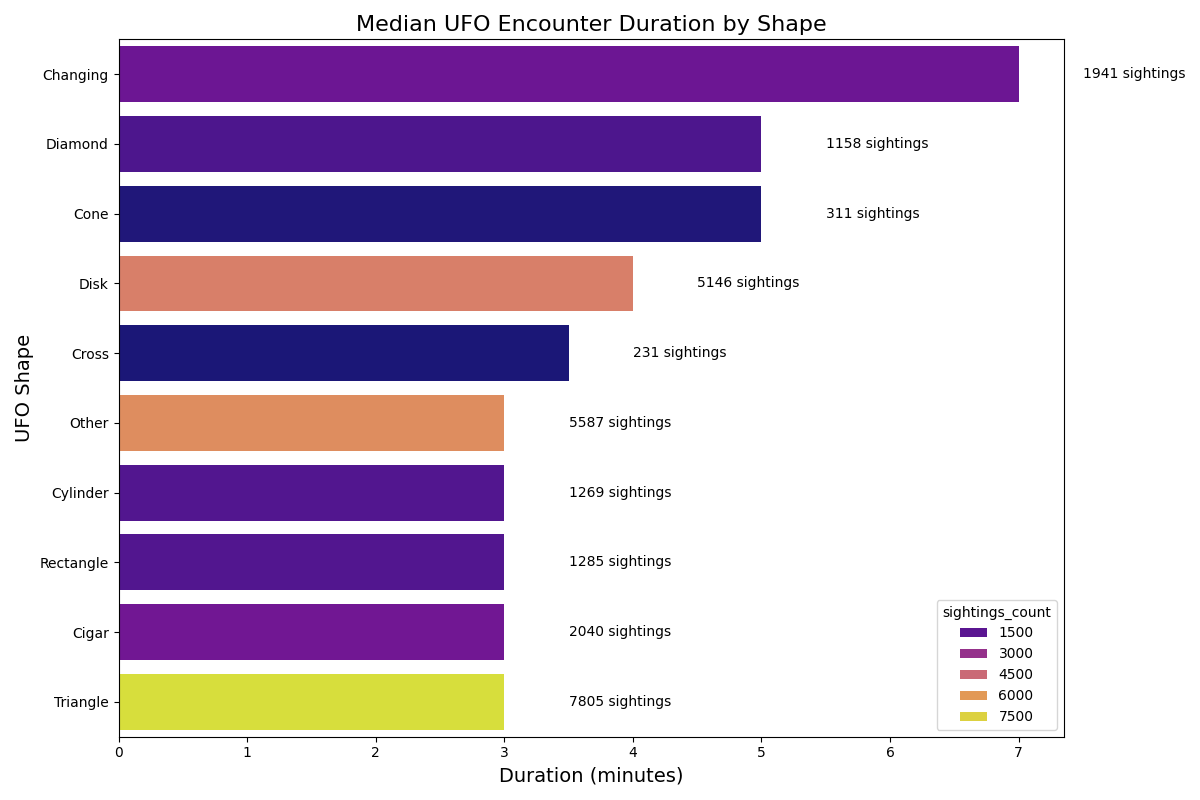
\includegraphics[width=0.8\textwidth]{../images/ufo_encounter_duration.png}
\caption{Délka pozorování UFO podle tvaru objektu}
\end{figure}

\subsection{Pozorování v průběhu dne a roku}
Třetí analýza zkoumala, jak se počet pozorování UFO mění v průběhu dne a roku. Použil jsem následující SQL dotaz:

\begin{lstlisting}[language=sql, caption=SQL dotaz pro počet pozorování podle měsíce a denní doby]
SELECT 
    CASE t.month
        WHEN 1 THEN 'January'
        WHEN 2 THEN 'February'
        WHEN 3 THEN 'March'
        WHEN 4 THEN 'April'
        WHEN 5 THEN 'May'
        WHEN 6 THEN 'June'
        WHEN 7 THEN 'July'
        WHEN 8 THEN 'August'
        WHEN 9 THEN 'September'
        WHEN 10 THEN 'October'
        WHEN 11 THEN 'November'
        WHEN 12 THEN 'December'
    END AS month,
    CASE
        WHEN t.hour >= 5 AND t.hour < 12 THEN 'Morning'
        WHEN t.hour >= 12 AND t.hour < 17 THEN 'Afternoon' 
        WHEN t.hour >= 17 AND t.hour < 22 THEN 'Evening'
        ELSE 'Night'
    END AS time_of_day,
    COUNT(*) AS sightings_count
FROM fact_sightings f
JOIN dim_time t ON f.time_id = t.time_id
GROUP BY t.month, time_of_day
ORDER BY 
    t.month,
    CASE 
        WHEN time_of_day = 'Morning' THEN 1
        WHEN time_of_day = 'Afternoon' THEN 2
        WHEN time_of_day = 'Evening' THEN 3
        WHEN time_of_day = 'Night' THEN 4
    END
\end{lstlisting}

Výsledky byly vizualizovány pomocí teplotní mapy (heatmap), která ukazuje počet pozorování v různých měsících a denních dobách:

\begin{figure}[h]
\centering
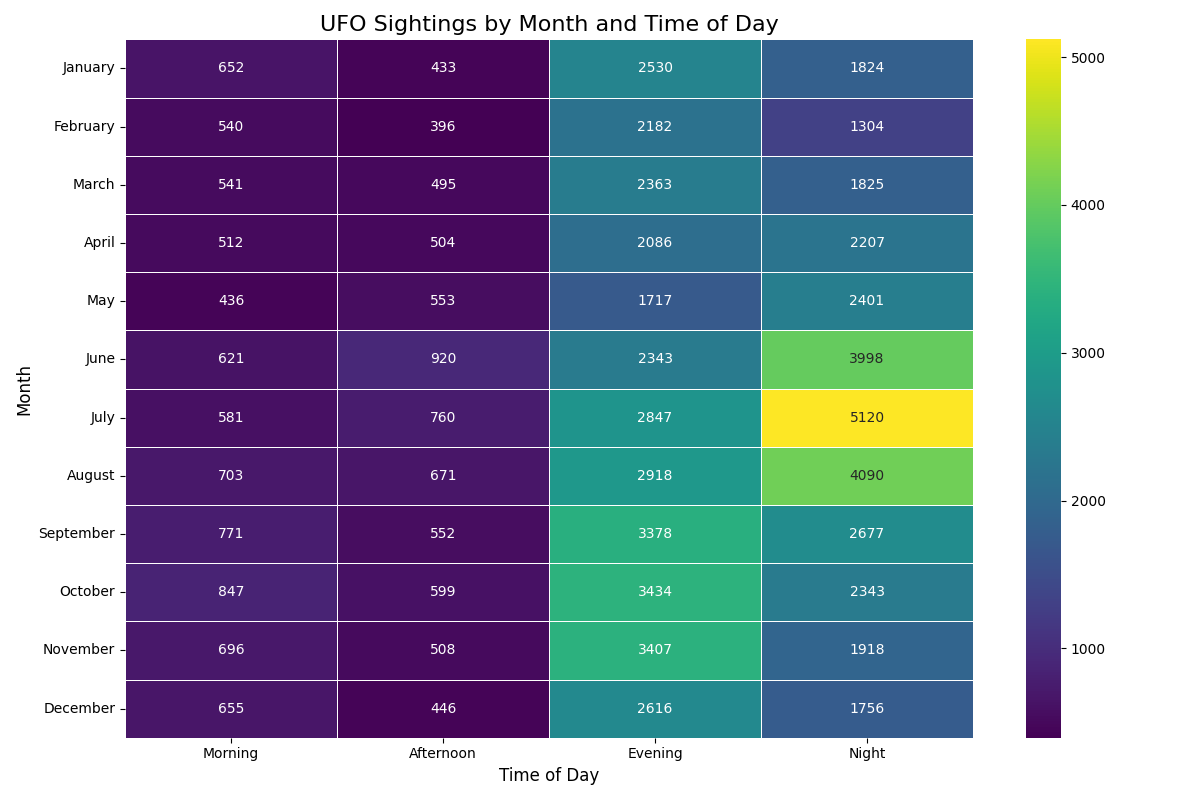
\includegraphics[width=0.8\textwidth]{../images/ufo_sightings_by_time.png}
\caption{Distribuce pozorování UFO podle měsíce a denní doby}
\end{figure}

\subsection{Analýza popisů pozorování}
Provedl jsem také analýzu textových popisů pozorování UFO, abych identifikoval nejčastější slova spojená s jednotlivými tvary objektů. Implementace zahrnovala předzpracování textu a využití knihovny Counter z modulu collections:

\begin{lstlisting}[language=python, caption=Kód pro analýzu textových popisů]
# SQL prikaz pro ziskani tvaru a popisku ufo
query = """
SELECT 
    d.ufo_shape,
    f.description
FROM fact_sightings f
JOIN dim_ufo d ON f.ufo_id = d.ufo_id
WHERE f.description IS NOT NULL 
  AND LENGTH(f.description) > 20
  AND d.ufo_shape IS NOT NULL
  AND d.ufo_shape != 'unknown'
LIMIT 10000
"""

# Funkce pro cisteni a tokenizaci textu
def clean_text(text):
    if not isinstance(text, str):
        return []
    # Prevod na mala pismena
    text = text.lower()
    # Odstraneni specialnich znaku a cislic
    text = re.sub(r'[^a-zA-Z\s]', '', text)
    # Tokenizace
    tokens = text.split()
    # Odstraneni stop slov (bezných slov, která neprinaseji velky vyznam)
    stop_words = {'the', 'and', 'to', 'of', 'a', 'in', 'that', 'it', '...'}
    tokens = [token for token in tokens if token not in stop_words and len(token) > 2]
    return tokens
\end{lstlisting}

Pro vizualizaci výsledků jsem vytvořil teplotní mapu (heatmap) a word cloudy pro nejčastější tvary UFO:

\begin{figure}[h]
\centering
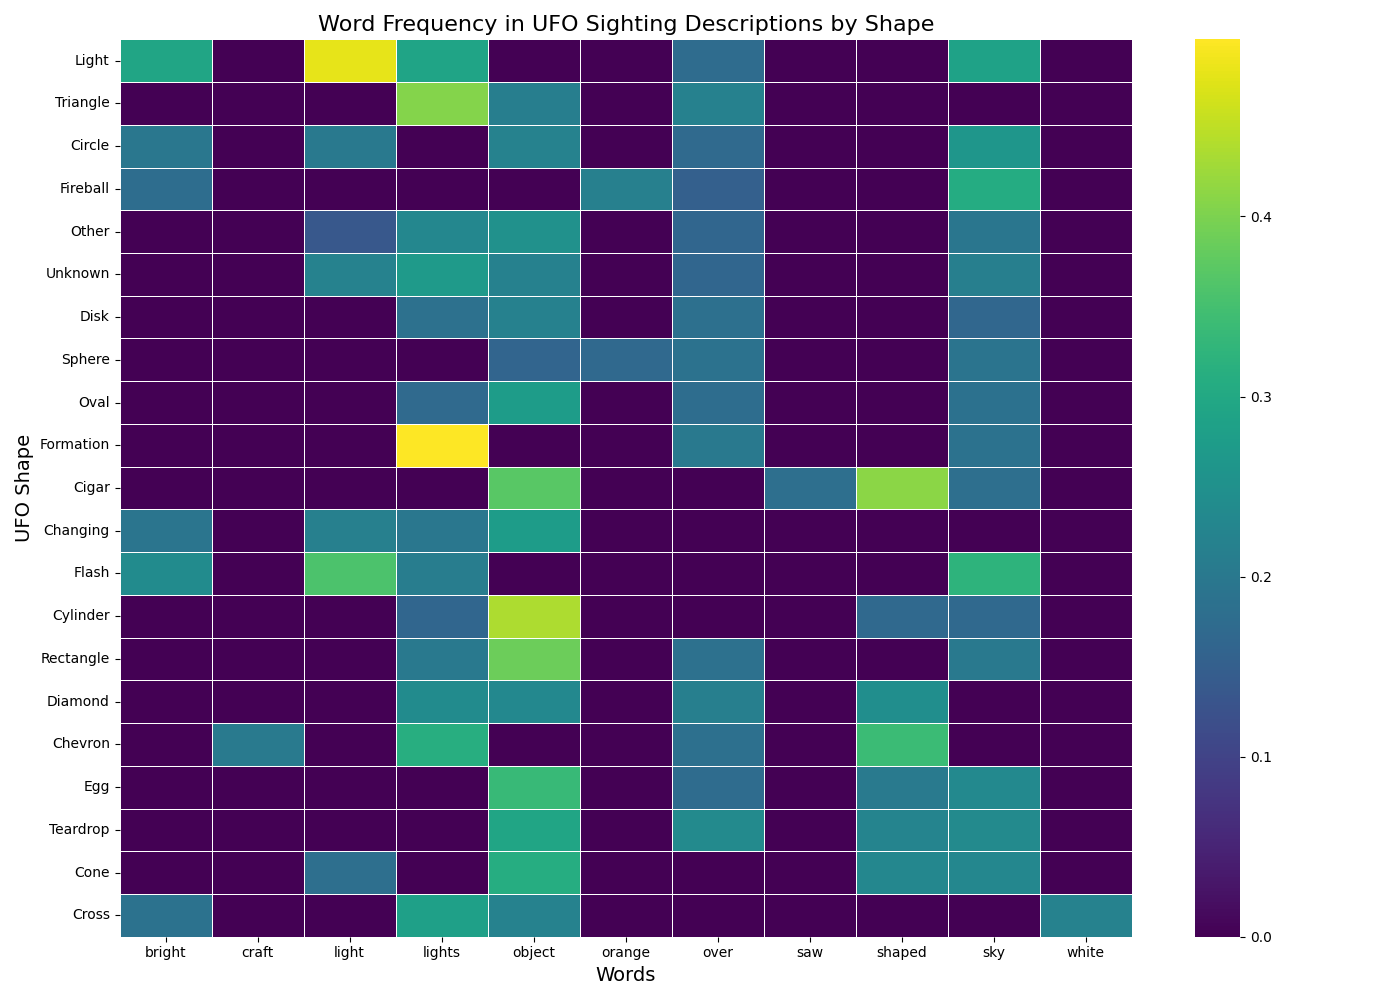
\includegraphics[width=0.8\textwidth]{../images/ufo_description_analysis.png}
\caption{Analýza slov v popisech pozorování UFO podle tvaru objektu}
\end{figure}

\begin{figure}[h]
\centering
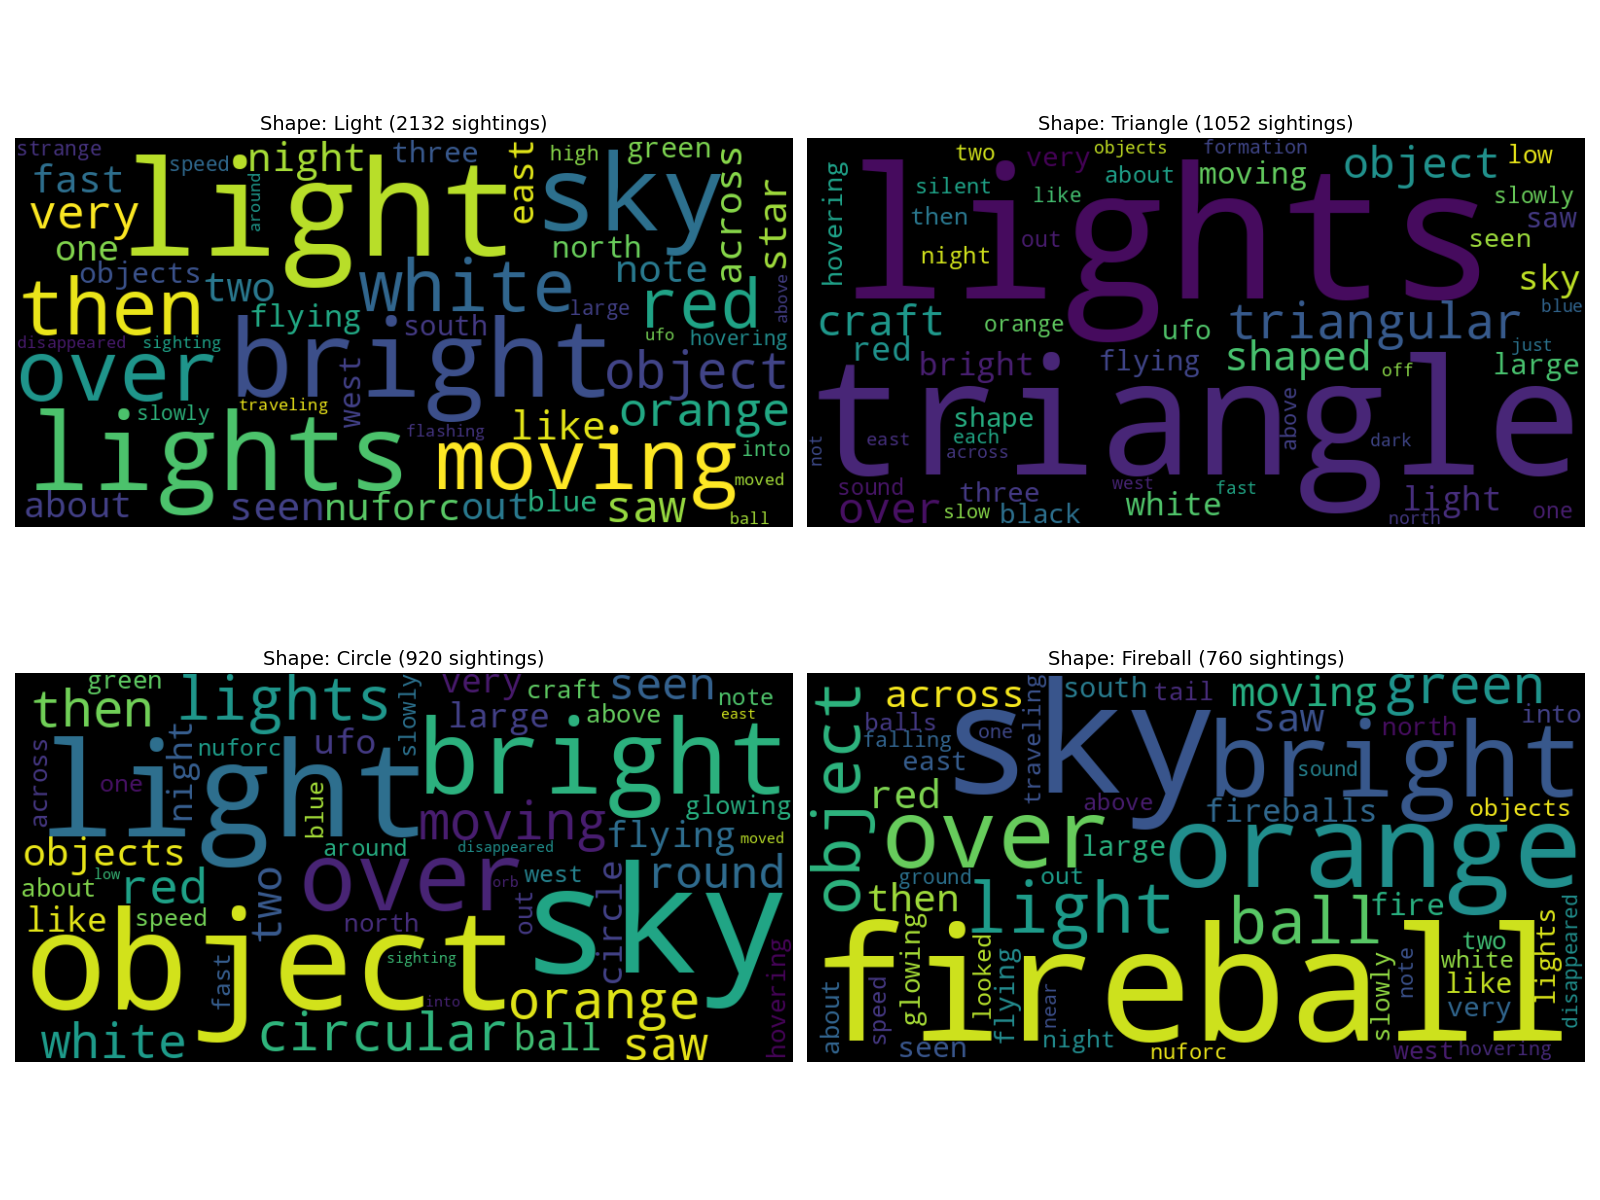
\includegraphics[width=0.8\textwidth]{../images/ufo_shape_wordclouds.png}
\caption{Word cloudy nejčastějších slov v popisech podle tvaru UFO}
\end{figure}

\section{Data mining}
Pro hlubší analýzu dat jsem použil metody dolování znalostí (data mining), které umožňují objevit skryté vzory a souvislosti v datech.

\subsection{Shlukování (Clustering)}
Použil jsem metodu K-Means clusteringu k identifikaci oblastí s podobnými charakteristikami pozorování UFO. Při shlukování jsem bral v úvahu geografickou polohu (zeměpisnou šířku a délku) a dobu trvání pozorování:

\begin{lstlisting}[language=python, caption=Implementace K-means shlukování]
# Priprava dat pro shlukovani
cluster_data = df[['latitude', 'longitude', 'length_of_encounter_seconds']].copy()

# Logaritmicka transformace doby trvani (protoze je obvykle zesikmena)
cluster_data['log_duration'] = np.log1p(cluster_data['length_of_encounter_seconds'])

# Standardizace přiznaku
scaler = StandardScaler()
scaled_features = scaler.fit_transform(cluster_data[['latitude', 'longitude', 'log_duration']])

# Urceni optimalního poctu shluku pomoci metody elbow
inertia = []
k_range = range(2, 11)
for k in k_range:
    kmeans = KMeans(n_clusters=k, random_state=42, n_init=10)
    kmeans.fit(scaled_features)
    inertia.append(kmeans.inertia_)

# Zvoleni konecneho poctu shluku
k = 5 
kmeans = KMeans(n_clusters=k, random_state=42, n_init=10)
clusters = kmeans.fit_predict(scaled_features)
\end{lstlisting}

Výsledky shlukování byly vizualizovány na mapě, která ukazuje rozložení jednotlivých shluků a jejich centra:

\begin{figure}[h]
\centering
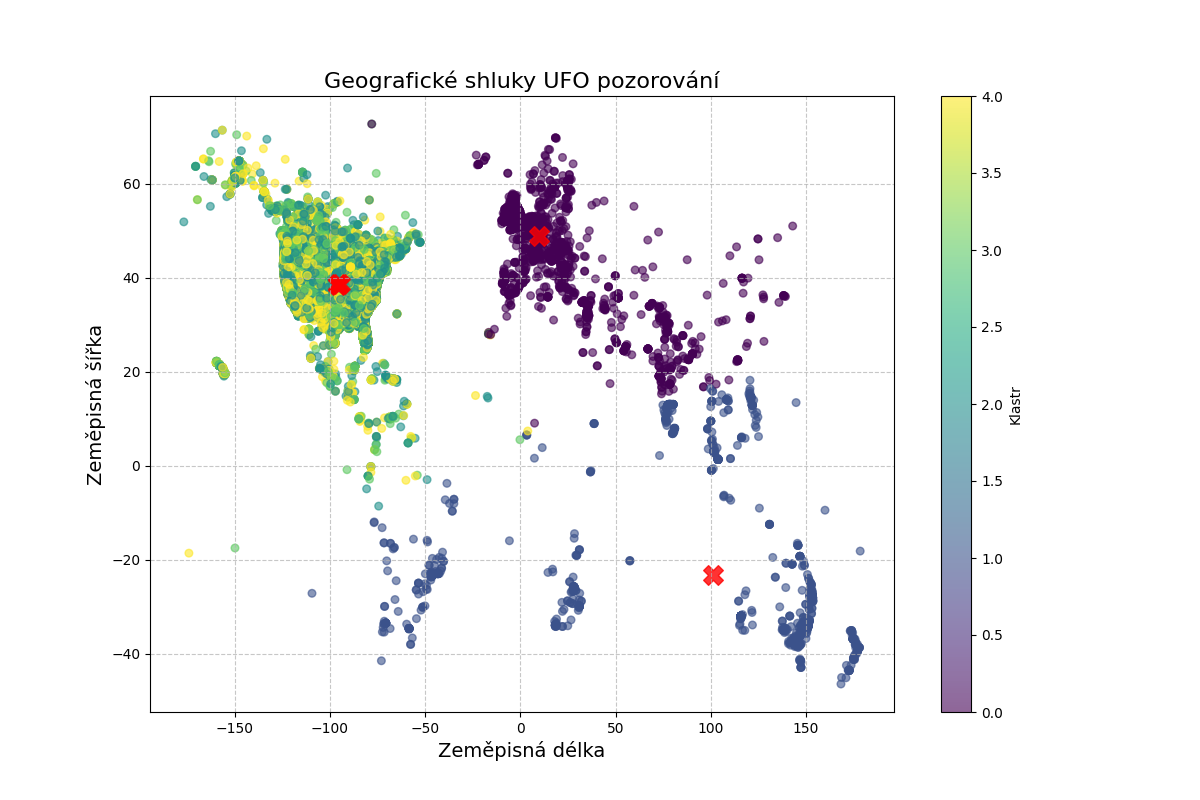
\includegraphics[width=0.8\textwidth]{../images/ufo_clusters_map.png}
\caption{Mapa shluků pozorování UFO}
\end{figure}

\begin{figure}[h]
\centering
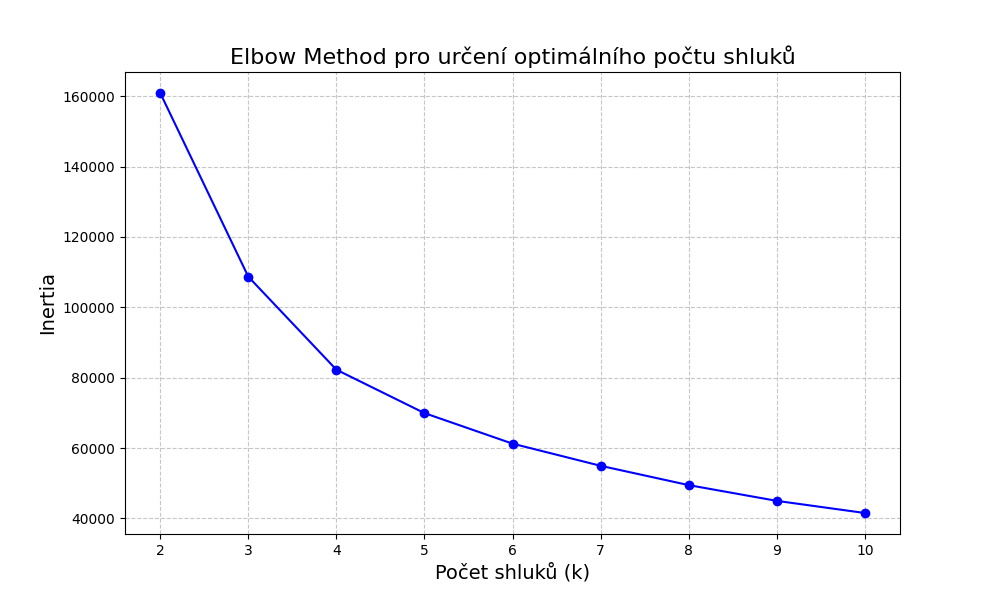
\includegraphics[width=0.8\textwidth]{../images/ufo_elbow_method.png}
\caption{Graf metody elbow pro určení optimálního počtu shluků}
\end{figure}

\subsection{Asociační pravidla}
Pro identifikaci zajímavých asociací v datech jsem použil algoritmus Apriori pro dolování asociačních pravidel. Tato metoda umožňuje objevit, které kombinace vlastností se často vyskytují společně:

\begin{lstlisting}[language=python, caption=Implementace dolování asociačních pravidel]
# Priprava kategorickych priznaku
categorical_features = ['ufo_shape', 'season', 'is_weekend']

# Pridáni diskretizovanych numerickych priznaku
df['duration_category'] = pd.cut(
    df['length_of_encounter_seconds'], 
    bins=[0, 60, 300, 900, 3600, 86400],
    labels=['<1min', '1-5min', '5-15min', '15min-1hr', '>1hr']
)

df['hour_category'] = pd.cut(
    df['hour'], 
    bins=[-0.1, 5.9, 11.9, 17.9, 23.9],
    labels=['night', 'morning', 'afternoon', 'evening']
)

categorical_features.extend(['duration_category', 'hour_category'])

# One-hot kodovani kategorickych priznaku
encoded_df = pd.get_dummies(df[categorical_features])

# Nalezeni castych itemsetu
min_support = 0.03  # Minimální podpora
frequent_itemsets = apriori(encoded_df, min_support=min_support, use_colnames=True)
frequent_itemsets['length'] = frequent_itemsets['itemsets'].apply(lambda x: len(x))

# Generovani asociacnich pravidel
min_threshold = 0.7  # Minimalni spolehlivost
rules = association_rules(frequent_itemsets, metric="confidence", min_threshold=min_threshold)

# Serazeni pravidel podle liftu
rules = rules.sort_values('lift', ascending=False)
\end{lstlisting}

Výsledky byly vizualizovány pomocí grafu scatter plot, který ukazuje vztah mezi podporou, spolehlivostí a liftem jednotlivých pravidel:

\begin{figure}[h]
\centering
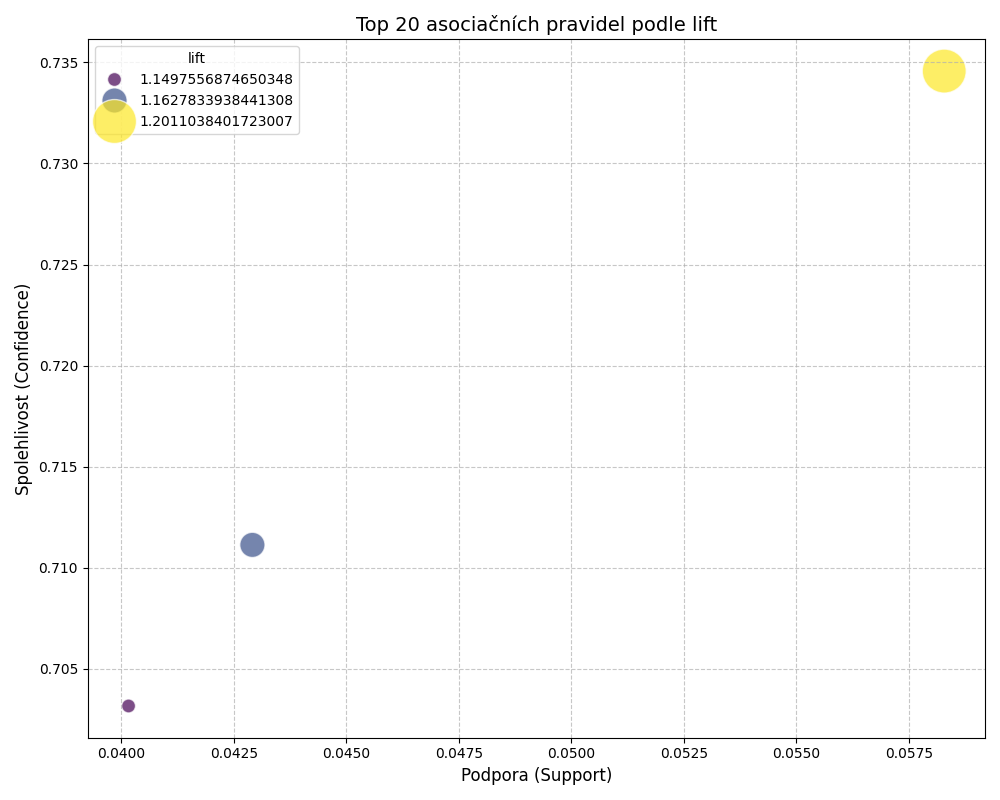
\includegraphics[width=0.8\textwidth]{../images/ufo_association_rules.png}
\caption{Asociační pravidla v datech o pozorování UFO}
\end{figure}

\begin{figure}[h]
\centering
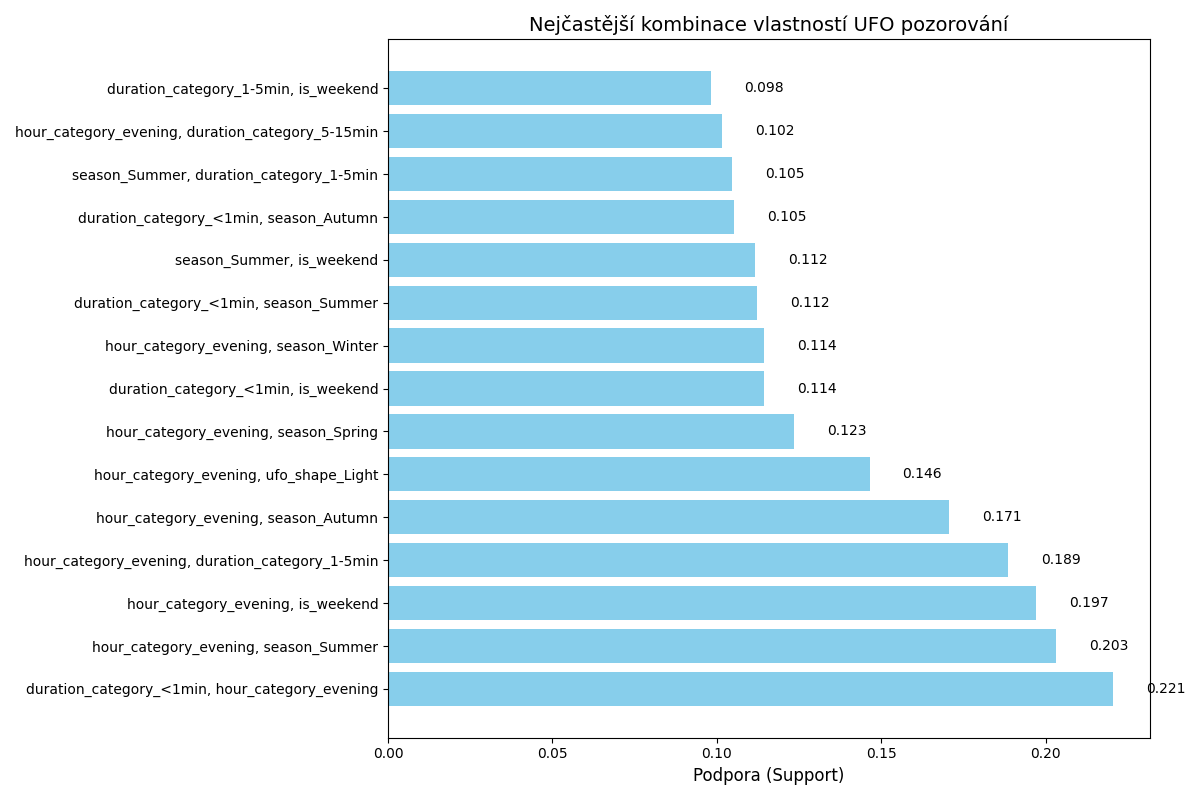
\includegraphics[width=0.8\textwidth]{../images/ufo_frequent_itemsets.png}
\caption{Nejčastější kombinace vlastností UFO pozorování}
\end{figure}

\FloatBarrier
\section{Závěr}
V tomto projektu jsem úspěšně demonstroval použití DuckDB pro OLAP analýzy na reálném datasetu o pozorováních UFO. DuckDB se ukázal jako výkonný a snadno použitelný nástroj pro analytické zpracování dat, který kombinuje jednoduchost použití s vysokým výkonem.

Hlavní přínosy projektu:

\begin{itemize}
    \item \textbf{Praktické použití DuckDB} - instalace, vytvoření databáze a provedení komplexních analytických dotazů
    \item \textbf{Vytvoření dimenzionálního modelu} - implementace struktury hvězdy (star schema) pro efektivní analytické dotazování
    \item \textbf{Implementace OLAP dotazů} - využití SQL a Python API pro analýzu dat z různých perspektiv
    \item \textbf{Aplikace metod data miningu} - využití shlukování a asociačních pravidel pro objevení skrytých vzorů v datech
    \item \textbf{Vizualizace výsledků} - vytvoření rozmanitých vizualizací pro lepší interpretaci získaných poznatků
\end{itemize}

Na základě analýz jsem zjistil několik zajímavých vzorů v datech o pozorováních UFO:

\begin{itemize}
    \item Kalifornie, Florida a Washington patří mezi státy s nejvyšším počtem hlášených pozorování UFO
    \item Většina pozorování se odehrává v nočních hodinách, přičemž v letních měsících je počet pozorování obecně vyšší
    \item Existují určité geografické shluky, které mají specifické charakteristiky z hlediska délky trvání a typu objektu
    \item Z analýzy textových popisů vyplývá, že určité tvary UFO jsou častěji spojovány s konkrétními slovy a popisy
\end{itemize}

DuckDB se osvědčil jako ideální nástroj pro tento typ analytických úloh díky své jednoduchosti, výkonu a schopnosti efektivně zpracovávat analytické dotazy bez nutnosti složité konfigurace.

Projekt je kompletně připraven v repozitáři a doplněn o vizualizace výsledků. Zdrojový kód je organizován do samostatných skriptů pro jednotlivé analýzy, což usnadňuje údržbu a rozšíření projektu v budoucnu.

\end{document}
